\documentclass[12pt,a4]{article}
\usepackage[english]{babel}
\usepackage[utf8]{inputenc}
\usepackage[T1]{fontenc}
\usepackage{geometry}
\usepackage{float}
\geometry{
	a4paper,
	left=20mm,
	right=20mm,
	top=20mm,
	bottom=20mm,
}
% Useful packages
\usepackage{amsmath}
\usepackage{bm}
\usepackage{graphicx}
\usepackage[colorlinks=true, allcolors=blue]{hyperref}

\begin{document}

\section{System matrices of the 6 DOF model}
\begin{equation}
	\bm{M} \bm{\dot{\nu}} + \bm{C}(\bm{\nu})\bm{\nu} + \bm{D}(\bm{\nu})\bm{\nu} = \bm{\tau}
\end{equation}
\begin{align}
	\bm{M} & = \bm{M}_{RB} + \bm{M}_A \\
	\bm{C} & = \bm{C}_{RB} + \bm{C}_A
\end{align}
\begin{equation*}
	\bm{\dot{\nu}} = \bm{A} \bm{\nu} + \bm{B} \bm{\tau}
\end{equation*}
In the case of no payload, no current and no external force $\tau$ we have

\begin{equation*}
	\bm{M}_{RB} = \left[\begin{array}{cccccc} 55 & 0 & 0 & 0 & -11 & 0\\ 0 & 55 & 0 & 11 & 0 & 11\\ 0 & 0 & 55 & 0 & -11 & 0\\ 0 & 11 & 0 & 14.6643 & 0 & 4.4000\\ -11 & 0 & -11 & 0 & 22.5500 & 0\\ 0 & 11 & 0 & 4.4000 & 0 & 18.1500 \end{array}\right]
\end{equation*}
\begin{multline*}
	\bm{C}_{RB} = \\
	\left[\begin{array}{cccccc} 0 & -55\,r & 55\,q & -11\,r & -11\,q & -11\,r\\ 55\,r & 0 & -55\,p & 0 & 11\,p-11\,r & 0\\ -55\,q & 55\,p & 0 & 11\,p & 11\,q & 11\,p\\ 11\,r & 0 & -11\,p & 0 & 4.4000\,p+13.7500\,r & -18.1500\,q\\ 11\,q & 11\,r-11\,p & -11\,q & -4.4000\,p-13.7500\,r & 0 & 10.2643\,p+4.4000\,r\\ 11\,r & 0 & -11\,p & 18.1500\,q & -10.2643\,p-4.4000\,r & 0 \end{array}\right]
\end{multline*}
\begin{equation*}
	\bm{M}_{A} = \left[\begin{array}{cccccc} 5.5000 & 0 & 0 & 0 & 0 & 0\\ 0 & 82.5000 & 0 & 0 & 0 & 0\\ 0 & 0 & 55 & 0 & 0 & 0\\ 0 & 0 & 0 & 2.4929 & 0 & 0\\ 0 & 0 & 0 & 0 & 14.5200 & 0\\ 0 & 0 & 0 & 0 & 0 & 27.1150 \end{array}\right]
\end{equation*}
\begin{equation*}
	\bm{C}_{A} = \left[\begin{array}{cccccc} 0 & 0 & 0 & 0 & 55\,w & -82.5000\,v\\ 0 & 0 & 0 & -55\,w & 0 & 5.5000\,u\\ 0 & 0 & 0 & 82.5000\,v & -5.5000\,u & 0\\ 0 & 55\,w & -82.5000\,v & 0 & 27.1150\,r & -14.5200\,q\\ -55\,w & 0 & 5.5000\,u & -27.1150\,r & 0 & 2.4929\,p\\ 0 & 0 & 0 & 14.5200\,q & -2.4929\,p & 0 \end{array}\right]
\end{equation*}
\begin{equation*}
	\bm{D} = \left[\begin{array}{cccccc} 77.5544 & 0 & 0 & 0 & 0 & 0\\ 0 & 0 & 0 & 0 & 0 & 0\\ 0 & 0 & 546.4805 & 0 & 0 & 0\\ 0 & 0 & 0 & 54.3823 & 0 & 0\\ 0 & 0 & 0 & 0 & 246.0496 & 0\\ 0 & 0 & 0 & 0 & 0 & 452.6500\,\left|r\right|+45.2650 \end{array}\right]
\end{equation*}


\section{Reduction from system equations}
\begin{equation}
	\dot{\bm{\nu}} = (\bm{M}_{RB}+\bm{M}_{A})^{-1}(-\bm{C}_{RB}-\bm{C}_{A}-\bm{D})\bm{\nu}
\end{equation}
\begin{equation}
	\dot{\bm{\nu}} = f(\bm{\nu}) = f(u, v, w, p, q, r)
\end{equation}
\begin{equation}
	\dot{\bm{\nu}} = \begin{bmatrix}\dot{u}&\dot{v}&\dot{w}&\dot{p}&\dot{q}&\dot{r}\end{bmatrix}^T
\end{equation}

\begin{multline}
	\dot{u} = 0.3371\,p\,r-1.3574\,u-0.2925\,w-1.3169\,q-0.0147\,p\,v-0.0265\,q\,u \\
	-1.8664\,q\,w+2.3477\,r\,v+0.2649\,u\,w+0.0177\,p^2+0.1866\,q^2+0.1690\,r^2
\end{multline}
\begin{multline}
	\dot{v} = 0.2504\,p+0.0651\,r-0.0364\,p\,q+0.1167\,q\,r+0.7867\,p\,w-0.4028\,r\,u \\
	-0.1266\,v\,w+0.6506\,r\,\left|r\right|
\end{multline}
\begin{multline}
	\dot{w} = 0.5354\,q\,u-0.0415\,u-5.1289\,w-0.0146\,p\,r-1.2581\,p\,v-0.7243\,q \\
	-0.0265\,q\,w+0.0412\,r\,v+0.1457\,u\,w-0.0903\,p^2-0.0974\,q^2-0.0071\,r^2
\end{multline}
\begin{multline}
	\dot{p} = 0.2244\,r-3.3993\,p-0.1257\,p\,q-0.5847\,q\,r+0.1266\,p\,w-0.3545\,r\,u \\
	+1.7190\,v\,w+2.2439\,r\,\left|r\right|
\end{multline}
\begin{multline}
	\dot{q} = 0.8539\,p\,r-0.4151\,u-1.6087\,w-7.2431\,q-0.0810\,p\,v-0.1457\,q\,u \\
	-0.2649\,q\,w+0.4121\,r\,v+1.4572\,u\,w+0.0971\,p^2+0.0265\,q^2-0.0707\,r^2
\end{multline}
\begin{multline}
	\dot{r} = 0.2696\,p-1.0376\,r-0.4188\,p\,q+0.1257\,q\,r+0.0395\,p\,w-0.1107\,r\,u \\
	-0.1363\,v\,w-10.3762\,r\,\left|r\right|
\end{multline}


\begin{multline}
	\bm{A} = \dfrac{df}{d\bm{\nu}}=	\\
	\left[\begin{array}{ccc}
			0.2649\,w-0.0265\,q-1.3574 & 2.3477\,r-0.0147\,p & 0.3371\,p+0.3379\,r+2.3477\,v \\
			-0.4028\,r                 & -0.1266\,w          & A_{23}                        \\
			-0.1107\,r                 & -0.1363\,w          & A_{33}
		\end{array}\right]
\end{multline}
Where the dimensions in heave, roll and pitch has been removed and
\begin{align}
	A_{23} & = 0.1167\,q+0.1301\,r-0.4028\,u	+1.3012\,\left|r\right|  \\
	A_{33} & = 0.1257\,q-2.0752\,r-0.1107\,u	-20.7524\,\left|r\right|
\end{align}
\begin{equation}
	\bm{B} = \left[\begin{array}{ccc} 0.0175 & 0 & 0\\ 0 & 0.0078 & -0.0014\\ 0 & -0.0014 & 0.0229 \end{array}\right]
\end{equation}

\subsection{Reduction}

Assiming that

\begin{align*}
	w & = 0 \\
	p & = 0 \\
	q & = 0
\end{align*}
The system equations simplify to
\begin{equation}
	\bm{A}(u,v,r)  = \left[\begin{array}{ccc}
			-1.3574    & 2.3477\,r & 0.3379\,r+2.3477\,v                        \\
			-0.4028\,r & 0         & 0.0651 -0.4028\,u		+1.3012\,\left|r\right|   \\
			-0.1107\,r & 0         & -1.0376 -0.1107\,u		-20.7524\,\left|r\right|
		\end{array}\right]
\end{equation}
\begin{equation}
	\bm{B} = \left[\begin{array}{ccc} 0.0175 & 0 & 0\\ 0 & 0.0078 & -0.0014\\ 0 & -0.0014 & 0.0229 \end{array}\right]
\end{equation}
Choosing the linearization point $(u,v,r) = (3,0,0)$ yields the following linearization
\begin{equation*}
	\bm{A} = \left[\begin{array}{ccc} -1.3574 & 0 & 0\\ 0 & 0 & -1.1433\\ 0 & 0 & -1.3696 \end{array}\right]
\end{equation*}
\begin{equation}
	\bm{B} = \left[\begin{array}{ccc} 0.0175 & 0 & 0\\ 0 & 0.0078 & -0.0014\\ 0 & -0.0014 & 0.0229 \end{array}\right]
\end{equation}



\section{Simple state truncation}


\begin{multline}
	\bm{A} =  -(M_{RB} + M_A)^{-1}(C_{RB}+C_A+D) = \\
	\left[\begin{array}{ccc}
			0.2944\,w-0.0294\,q-1.3574 & 0.0294\,p+0.9037\,r & 0.1690\,r-0.0742\,p+1.4439\,v                      \\
			-0.3601\,r                 & 0.2532\,w           & 0.6506\,\left|r\right|-0.0427\,u-0.1504\,q+0.0651  \\
			-0.1186\,r                 & 0.2726\,w           & 0.0079\,u-0.1620\,q-10.3762\,\left|r\right|-1.0376
		\end{array}\right]
\end{multline}
\begin{equation}
	\bm{B} = (M_{RB} + M_A)^{-1}=  \\
	\left[\begin{array}{ccc}
			0.0175 & 0       & 0       \\
			0      & 0.0078  & -0.0014 \\
			0      & -0.0014 & 0.0229
		\end{array}\right]
\end{equation}
where the heave, roll and pitch dimensions has been removed from \textit{A} and \textit{B}

\subsection{Reduction}

Assiming that

\begin{align*}
	w & = 0 \\
	p & = 0 \\
	q & = 0
\end{align*}
The system equations simplify to
\begin{equation*}
	\bm{A}(u,v,r) =
	\left[\begin{array}{ccc}
			-1.3574    & 0.9037\,r & 0.1690\,r+1.4439\,v                      \\
			-0.3601\,r & 0         & 0.6506\,\left|r\right|-0.0427\,u+0.0651  \\
			-0.1186\,r & 0         & 0.0079\,u-10.3762\,\left|r\right|-1.0376
		\end{array}\right]
\end{equation*}
\begin{equation*}
	\bm{B} =
	\left[\begin{array}{ccc}
			0.0175 & 0       & 0       \\
			0      & 0.0078  & -0.0014 \\
			0      & -0.0014 & 0.0229
		\end{array}\right]
\end{equation*}


\section{Selection matrix approch}

\begin{align}
	C^*_{RB} & = UM_{RB}L
	         &
	C^*_{A}  & = UM_AL
\end{align}
Where \textit{U} is the surge of the vessel at the linarization point and L is a selection matrix seen in HMCHMC (3.63).
For this lineariztion $U=3$
\begin{align}
	M_{RB} & = \left[\begin{array}{ccc} 55 & 0 & 0\\ 0 & 55 & 11\\ 0 & 11 & 18.1500 \end{array}\right]
	       &
	M_{A}  & = \left[\begin{array}{ccc} 5.5000 & 0 & 0\\ 0 & 82.5000 & 0\\ 0 & 0 & 27.1150 \end{array}\right]
\end{align}
\begin{align}
	C^*_{RB} & = \left[\begin{array}{ccc} 0 & 0 & 0\\ 0 & 0 & 165\\ 0 & 0 & 33 \end{array}\right]
	         &
	C^*_{A}  & = \left[\begin{array}{ccc} 0 & 0 & 0\\ 0 & 0 & 247.5000\\ 0 & 0 & 0 \end{array}\right]
\end{align}
\begin{equation}
	D = \left[\begin{array}{ccc} 77.5544 & 0 & 0\\ 0 & 0 & 0\\ 0 & 0 & 452.6500\,\left|r\right|+45.2650 \end{array}\right]
\end{equation}

\begin{equation}
	\dot{\nu} = A \nu + B \tau
\end{equation}

\begin{align}
	M & = M_{RB} + M_A            \\
	N & = C^*_{RB} + C^*_{A} + D* \\
	A & = -M^{-1}N                \\
	B & = M^{-1}
\end{align}

\begin{equation*}
	A = \left[\begin{array}{ccc} -1.2819 & 0 & 0\\ 0 & 0 & 0.8159\,\left|r\right|-2.9184\\ 0 & 0 & -10.1983\,\left|r\right|-1.0198 \end{array}\right]
\end{equation*}
\begin{equation*}
	B = \left[\begin{array}{ccc} 0.0165 & 0 & 0\\ 0 & 0.0074 & -0.0018\\ 0 & -0.0018 & 0.0225 \end{array}\right]
\end{equation*}





\section{Waterfixed coordinates}
In the common system equations $\nu$ is defined relative to the seabed
\begin{align}
	\bm{M}_{RB}\bm{\dot{\nu}} + \bm{M}_{A}\bm{\dot{\nu_r}} + \bm{C}_{A}(\bm{\nu})\bm{\nu} + \bm{C}_{RB}(\bm{\nu}_r)\bm{\nu}_r + \bm{D}(\bm{\nu}_r)\bm{\nu}_r & = \bm{\tau} + \bm{w}(t) \\
	\bm{\dot{\eta}}                                                                                                                                          & = \bm{J}(\eta)\bm{\nu}
\end{align}
If the velocities $\nu$ is defined relative to the water $\nu = \nu_r$. Since it is still preferred to have the position in land relative coordinates the velocities from the current needs to be included in the second equation.
\begin{align}
	\left(\bm{M}_{RB} + \bm{M}_{A}  \right) \bm{\dot{\nu}} + \left(\bm{C}_{A}(\bm{\nu}) + \bm{C}_{RB}(\bm{\nu}) + \bm{D}(\bm{\nu})  \right)\bm{\nu} & = \bm{\tau} + \bm{w}(t)             \\
	\bm{\dot{\eta}}                                                                                                                                 & = \bm{J}(\eta)\bm{\nu} + \bm{\nu}_c
\end{align}
Where $\bm{\nu}_c$ is the velocity vector of the current
\begin{equation}
	\bm{\nu}_c =  \begin{bmatrix}u_c & v_c & 0 & 0 & 0 & 0 \end{bmatrix}^T
\end{equation}


\section{Crossflow damping}



\begin{figure}[H]
	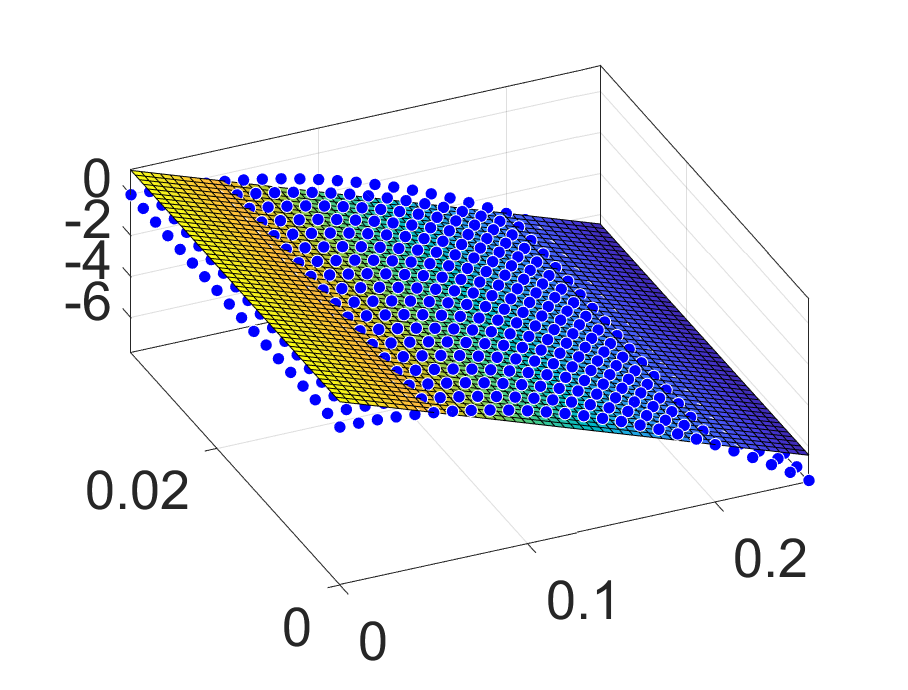
\includegraphics{graphics/SwayDampingLinearized.eps}
	\caption{Linearized crossflow damping in sway}
	\label{fig:SwayDampingLinearized}
\end{figure}
\begin{figure}[H]
	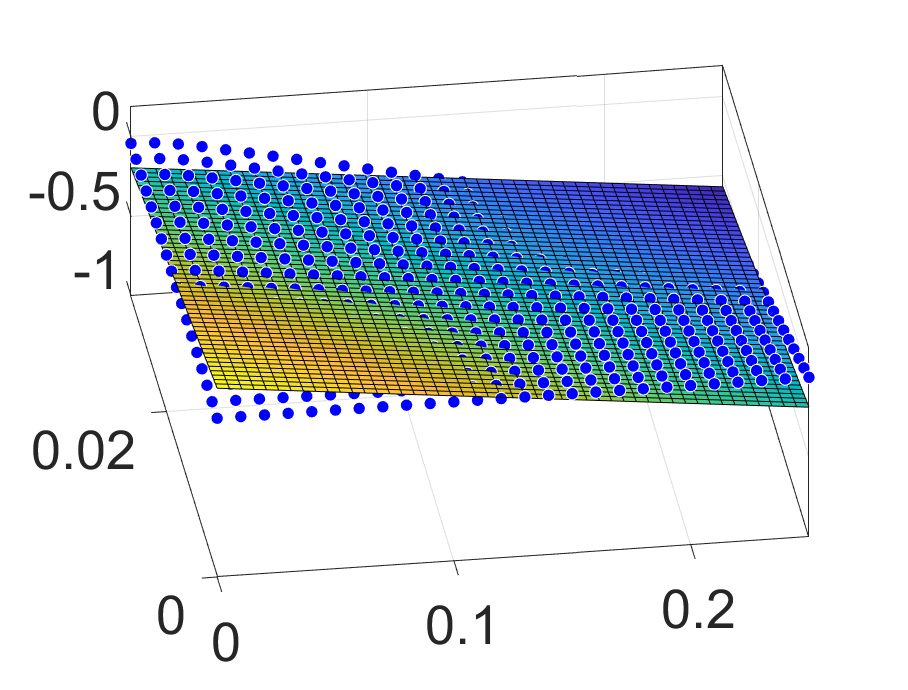
\includegraphics{graphics/YawDampingLinearized.eps}
	\caption{Linearized crossflow damping in yaw}
	\label{fig:YawDampingLinearized}
\end{figure}
\begin{equation*}
	\bm{\tau}_{cf} = \left[\begin{array}{c} 0\\ 1.2336-30.6073\,v-1.4439\,r\\ 0\\ 0\\ 0\\ 0.1891-1.5099\,v-11.2817\,r \end{array}\right]
\end{equation*}
\begin{multline*}
	\bm{D} = \dfrac{d}{d\bm{\nu}} (-\bm{\tau}_d-\bm{\tau}_{cf}) = \\
	= \left[\begin{array}{cccccc} 77.5544 & 0 & 0 & 0 & 0 & 0\\ 0 & 30.6073 & 0 & 0 & 0 & 1.4439\\ 0 & 0 & 546.4805 & 0 & 0 & 0\\ 0 & 0 & 0 & 54.3823 & 0 & 0\\ 0 & 0 & 0 & 0 & 246.0496 & 0\\ 0 & 1.5099 & 0 & 0 & 0 & 905.3000\,\left|r\right|+56.5467 \end{array}\right]
\end{multline*}

\end{document}
